\section{Accepted Medium-Campaign Diagnostics}
\label{app:medium_diagnostics}

These figures support the bounded observations in \Cref{sec:medium_evidence}. All use the accepted 75-cell campaign; no historical reduced diagnostic or external-testbed result is pooled into them. G, EXP, CP, and iCP denote GNeuralUCB, EXPNeuralUCB, CPursuitNeuralUCB, and iCPursuitNeuralUCB. The main-body trajectory and action-exposure plots are not repeated here.

\begin{figure*}[t]
\centering
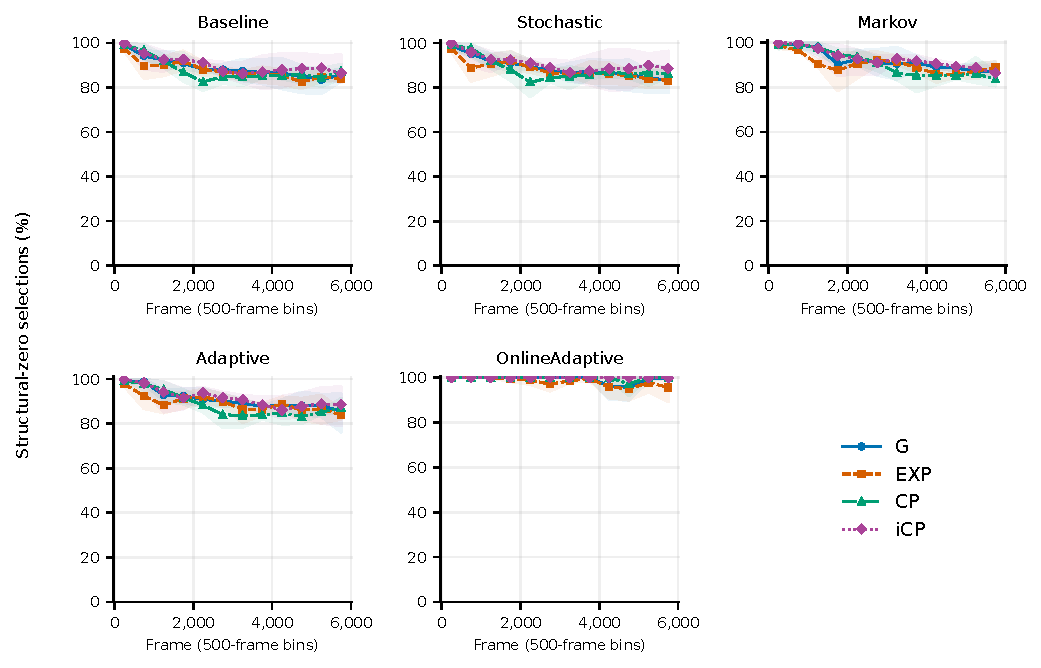
\includegraphics[width=\textwidth]{figures/icnp/medium_structural_zero.pdf}
\caption{Structural-zero action occupancy in twelve disjoint 500-frame bins. Lines are equal-block means; shading is the three-block min--max range, not a confidence interval. A structural-zero action has catalog base payoff exactly zero, irrespective of availability; the denominator is 500 selections per block/bin. Axis limits differ across threats. Changing occupancy is descriptive and does not isolate the cause of action selection or establish convergence.}
\label{fig:medium_structural_zero}
\end{figure*}

\begin{figure*}[t]
\centering
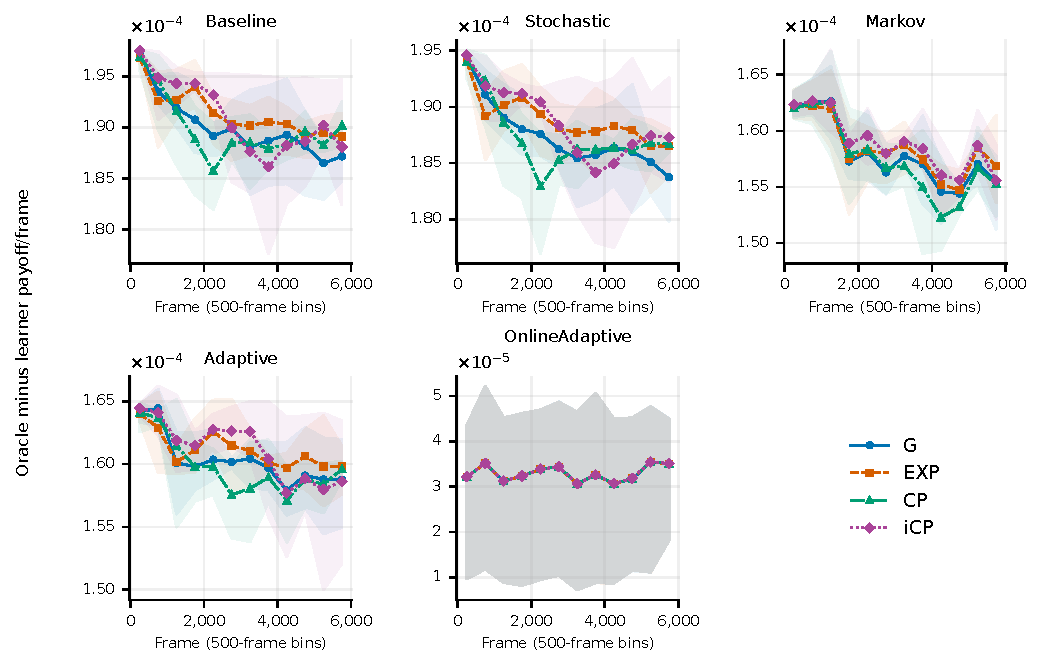
\includegraphics[width=\textwidth]{figures/icnp/medium_oracle_gap.pdf}
\caption{Descriptive Oracle gap in twelve disjoint 500-frame bins. The gap is mean Oracle continuous payoff minus mean learner continuous payoff per frame within the matched block/bin, not a percentage-point efficiency gap. Lines are equal-block means; shading is the three-block min--max range, not a confidence interval; axis limits differ across threats. Oracle has privileged payoff/availability information and, under reactive threats, its own induced history. Neither visual flattening nor a narrowing gap establishes convergence or an isolated cause of compression.}
\label{fig:medium_zero_gap}
\end{figure*}

\begin{figure*}[t]
\centering
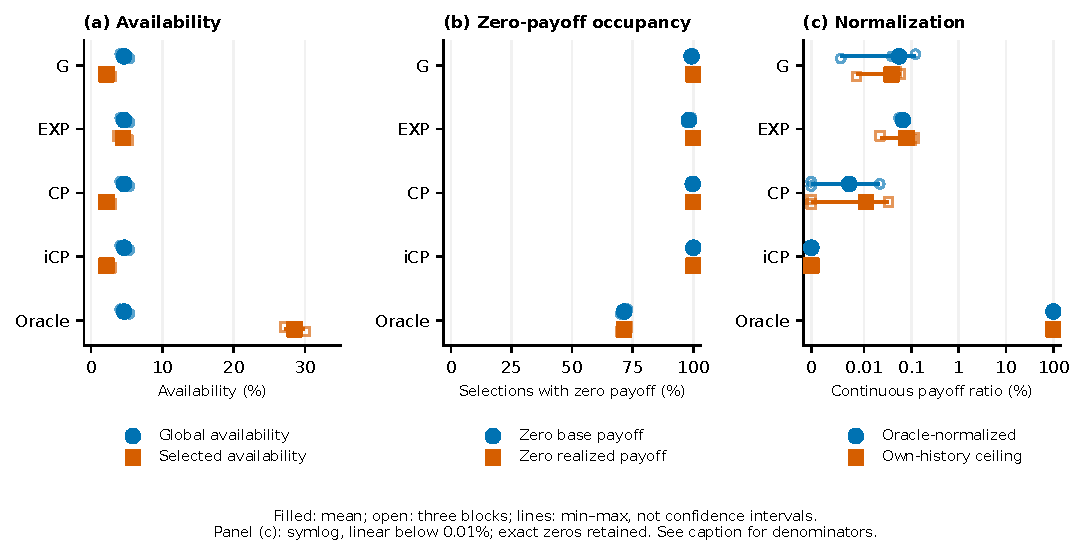
\includegraphics[width=\textwidth]{figures/icnp/medium_onlineadaptive.pdf}
\caption{OnlineAdaptive availability, action quality, and comparator sensitivity. Filled markers are equal-block means, open markers are the three blocks, and lines are min--max, not confidence intervals. Global availability uses 60,000 route-frames per block; selected availability and zero occupancy use 6,000 selections. Structural-zero selections are included in realized-zero selections, not additive causes. Panel (c) reports $100\sum_t u_t/\sum_t u_t^{\rm Oracle}$ and $100\sum_t u_t/\sum_t\max_{r,x}[q_r(x)A_t(r)]$, respectively: the latter uses each policy's recorded availability history, not a counterfactual trajectory. Ratios are calculated per block before averaging. The symlog axis is linear below 0.01\%; zeros are exact, with no positive offset. Oracle sees catalog payoffs/current availability and has a separate reactive history; its fallback choices when all routes are down do not imply avoidable poor-action selection. Equal global totals do not imply equal masks or causal comparability.}
\label{fig:medium_onlineadaptive}
\end{figure*}

\begin{figure*}[t]
\centering
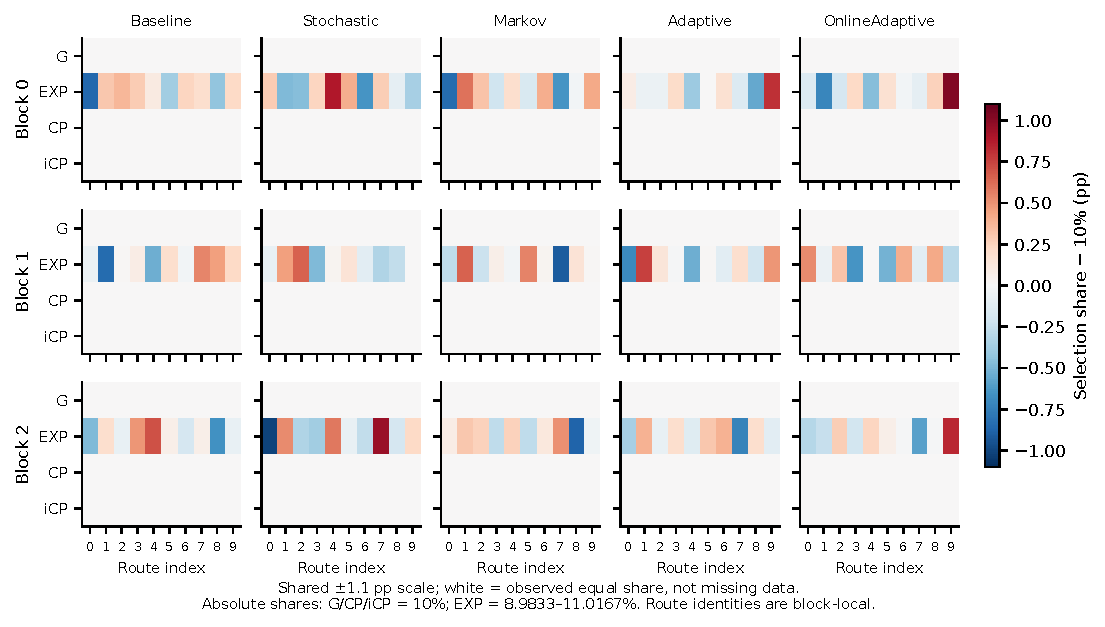
\includegraphics[width=\textwidth]{figures/icnp/medium_route_exposure.pdf}
\caption{Full-horizon route selection by original block and threat, centered on a 10\% equal-share reference with one shared $\pm1.1$ percentage-point scale. Each share divides route selections by 6,000 decisions. Route identities are block-local and are not pooled across blocks. White denotes observed zero deviation, not missing data. G/CP/iCP select each route 600 times per cell (10\%); EXP shares range from 8.9833\% to 11.0167\%. The reference is neither an optimal/fair allocation nor a statistical null model. Full-horizon totals do not establish temporal uniformity, random selection, absence of learning, or a route-selection mechanism.}
\label{fig:medium_route_exposure}
\end{figure*}
